\subsubsection{Logic Layer - Overview}
The Logic Layer consists of a Task Planner and its related methods, and classes to implement States, Modules and State Priority Queues

\subsubsection{Logic Layer - Task Planner}
The Task Planner begins by verifying the start and goal states have the same number and composition of modules; And generates states utilising the State Priority Queue and State Classes. It returns an array of states representing the transitions required to reconfigure the start state into the goal state.
\\\\
The Planner consists of two main methods, \textbf{“FindPath()“} and \textbf{“GenNewStates()”}. The \textbf{“FindPath()“} method implements the search algorithm shown in listing \ref{SearchPseudo}), while \textbf{“GenNewStates()”} expands the tree based on the heuristics specified in the design section \ref{genStates}, as can be seen in listing \ref{generateStatesPseudo}. After generating states, “FindPath()” records their parent states, enabling the program to trace the transition path from the starting state to the goal state.

\begin{lstlisting}[caption={State Generation Pseudo-code},captionpos=b,label={generateStatesPseudo}]
GenNewStates(state, goalState)
	stateQueue <- new StateQueue(goalState) 
	from <- state.getNonFinalModules()
	to <- state.getAvailablePositions()
	
	stateQueue.push(state.GenerateMoves(from, to))
	
	IF stateQueue.empty() DO:
		from <- state.getAdjacentModules(b)
		stateQueue.push(state.GenerateMoves(from, to))
	END
	
	IF stateQueue.empty() DO:
		from <- state.getModules()
		stateQueue.push(state.GenerateMoves(from, to))
	END
	RETURN stateQueue
\end{lstlisting}

\subsubsection{Logic Layer - State Priority Queue Class}
The State Priority Queue class maintains a sorted list of states using a simple array data structure. States are ordered based on their proximity to the goal state, as determined by the heuristics detailed in design section \ref{statePriority}. When a state is inserted, a binary search algorithm \cite{lin2019binary} is used to find the appropriate position in the queue to maintain the queue's priority order. Initially, a linear search algorithm was used for simplicity, but during optimization, the binary search was implemented, significantly reducing the overall insertion time.

\subsubsection{Logic Layer - State Class}
The State Class represents a state configuration and stores module positions. It includes methods for state comparisons, measurements, validation, and visualization. Modules are stored in a dictionary, where keys represent module positions and values are module objects.
\\\\
Initially, a position matrix was used for its simplicity in testing and modifying logic, which sped up development. However, it was later replaced by a dictionary for optimisation as unlike a position matrix, dictionaries do not store unnecessary zero values so increase memory efficiency of the system.
The class includes a verification function to ensure all modules in the state are connected.
\\\\
Originally, an out-of-the-box labelling algorithm from the scikit-image python package \cite{scikit-image} was used with the position matrix to verify connectivity. After switching to a dictionary, a new search algorithm was implemented for state verification (shown in listing \ref{verifyPseudo}).
\\\\
\begin{lstlisting}[caption={State Verification Pseudo-code},captionpos=b,label={verifyPseudo}]
VerifyState(state)
	foundList <- []
	searchList <- [state.getFirstModule()]
	WHILE searchList NOT empty DO:
		module <- searchList.pop()
		For neighbour in module.getNeighbours() DO:
		IF neighbour NOT in foundList DO:
			IF neighbour NOT in searchList DO:
				searchList.push(neighbour)
			END
		END
	END
	RETURN foundList.length() EQUALS state.numModules()
\end{lstlisting}
Several functions are implemented to measure the number of modules in final positions, the number of modules in free positions and the Euclidean distance between all modules in non-final positions and their final positions. Since these measurements are often requested multiple times for the same state, the calculated values are saved within the state after the initial computation and updated only if the goal state changes.
\\\\
For visualising reconfigurations and aiding in-depth testing and analysis, the State Class includes a display function. This function translates the dictionary into a position matrix, which is then displayed as a 3D matrix using Matplotlib \cite{Hunter2007}. Configurations, such as the one shown in figure \ref{stateVisual}, can be visualised. Additionally, this function is used to create reconfiguration videos, enabling clear visualisation of the system's output.
\begin{figure}[H]
	\centering
	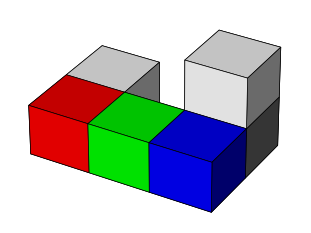
\includegraphics[width=0.5\textwidth]{state.png}
	\caption{State Visualisation}
	\label{stateVisual}
\end{figure}

As shown in listing \ref{generateStatesPseudo}, the State Class includes a function called \textbf{'GenerateMoves()'} for generating a list of states for mass movement of modules. This function takes two lists: one of module positions and another of positions the modules can move to. For each module, the function validates the state without the moving module to ensure the state remains intact during movement. It then moves the module to each of the possible positions, adding the new state to a return list if the state is valid after the movement. This custom mass movement function optimizes state generation during search tree expansion.

\subsubsection{Logic Layer - Module Class}
The Module Class is a straightforward class that holds information about a module, primarily used for comparing modules through an \textbf{"Equals()"} function. This function can be modified to adjust which module properties determine equality. In its current implementation, colour is used to decide if two modules are equal. There is functionality to compare by module type or module identification number. However, comparing by colour simplifies analysis during testing, as it allows for visual differentiation of modules when displayed.